\documentclass[12pt]{article}
\usepackage[margin=1in]{geometry}
\usepackage{hyperref}
\usepackage{indentfirst}
\usepackage[style=authoryear, maxcitenames=2, backend=biber]{biblatex}
\usepackage{graphicx}
\usepackage{float}
\usepackage{listings}
\usepackage{subcaption}
\usepackage{titling}
\setlength{\droptitle}{-4em}
\usepackage[font=small,labelfont=bf]{caption}

% Settings for equation formatting
\lstset{
  language=Python,
  basicstyle=\fontfamily{cmtt}\selectfont\small,
  keywordstyle=\color{purple},
  stringstyle=\color{red},
  commentstyle=\color{green!50!black},
  numbers=none,
  frame=single,
  breaklines=true,
  showstringspaces=false,
  columns=fullflexible,
  keepspaces=true,
  float=H,
  belowskip=0pt,
}

\addbibresource{references.bib}

\title{Köppen-Geiger Sentinel-2 Satellite Climate Classification}

\author{Abhijit Goda, Brian Salchert}

\date{24 April 2026}

\begin{document}

\maketitle

\centering
Project GitHub Repository: \url{https://github.com/Obby-108/KoppenSatelliteClimateClassification}

\abstract

Anthropogenic climate change poses serious risks for both human populations and natural ecosystems.
As changes in temperature (and by extension changes in weather and vegetation) continue to accelerate, there is an increasing need for reliable methods of tracking and quantifying changes to climates over time.
This project explores the use of multi-class classification models to assign one of thirty Köppen-Geiger climates to each area of the globe.
The use of high-resolution Sentinel-2 spectral data captures key environmental features, even in remote locations where collection of empirical data for classification is challenging or impossible.
We apply and evaluate several architectures, such as Convolutional Neural Networks (CNNs), One-versus-Rest Support Vector Machines (OvR SVMs), and ensemble methods, including Random Forests and Gradient Boosting.
These architectures provide the ability to capture both local features on climate boundaries and larger global features necessary for accurate classification.
In conducting a meticulous analysis and comparison of these models, this project aims to provide tools for generating high quality insights for quantifying the rate of climate change.
These findings provide the foundation for assessing natural disaster risk, informing urban planning decisions, improving agricultural yields, and more.

\section{Introduction}
\label{sec:introduction}

\indent We plan to address the issue of climate classification in the context of the Köppen-Geiger classification schema.
This schema is key to identifying the weather conditions of locations all around the world and for meteorological insights, using robust empirical methods to assign one out of thirty climates to every location across the globe.
However, there tend to be lots of difficulties in doing so especially in regions where data is inaccessible, like regions in the middle of the Sahara where data collection stations are sparse, or in dense tropical rainforests and developing nations, where maintaining such infrastructure is not feasible.

Rather, we extend the original motivation Wladimir Köppen had in developing his climate classification schema.
In the late 19th century, he realized vegetation boundaries are a natural proxy for climate zones.
This is because the ground is an inherent integrator of temperature and precipitation, affecting its topography, soil moisture, vegetation, and so on.

Historically, updating global maps based on Köppen's schema has relied on interpolation, such as that of Kriging, between unevenly distributed ground weather stations.
This skips over microclimates in between and fails to capture differences in between climate boundaries.
Rather, we propose the use of Sentinel-2 spectral data that comes in high resolution (10m to 60m per pixel), immense quantities, and with bands like Red Edge and Short-Wave Infrared (SWIR) that are sensitive to relevant land qualities, like vegetation health.
The work by \textcite{data-driven-kg} further justifies this approach, showing that data-driven methods provide a potentially more objective means of climate classification.
By training a model to associate spectral bands directly to Köppen-Geiger classes, we can create a much more granular, malleable climate map offering high-resolution insights for climate change, agriculture, and urban planning.

\section{Proposed Project}
\label{sec:proposed-project}

\indent Our specific problem context is figuring out how to transform multi-spectral data from the Sentinel-2  satellite into one of 30 Köppen-Geiger classes.
The dataset is synthesized in multiple steps from multiple sources.
First, using the high-resolution Köppen-Geiger GeoTIFF map uploaded to the Google Earth Engine Console, we randomly sampled 2,000 coordinates for each of the 30 climate classes from across the world, ensuring as little bias as possible across class samples, for a total of 60,000 coordinates.
These were saved as integers (for the climate classification) and latitude-longitude pairs in the GeoJSON string format.
Next, using the coordinates, we sampled 129 x 129 pixel patches of land centered about these coordinates, ensuring no overlap between close-by coordinates, and collected the 12 spectral bands, or in other words, reflection intensity of a satellite light wavelength (like Red Edge or Blue Edge), corresponding to each of the pixels in this patch.
In the end, this yielded 60,000 129 x 129 x 12 tensors, where each vertical 129 x 129 x 1 layer corresponded to a 129 x 129 collection of wavelength intensities for a single spectral band, all in the context of some 1.29 km patch of land somewhere in the world.
Extracting and plotting the three bands of visible light wavelengths for a particular sample from the data yields the plot in Figure~\ref{fig:sample-plot} below.

\begin{figure}[htbp]
  \centering
  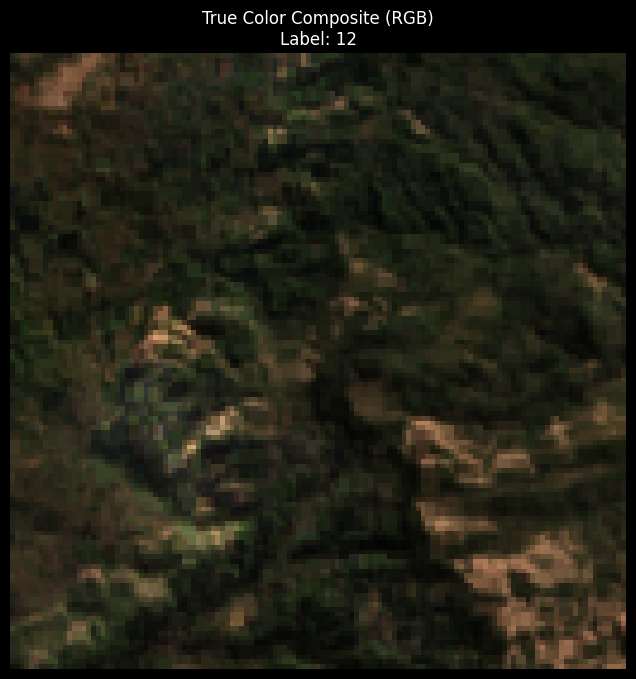
\includegraphics[width=0.4\textwidth]{sample}
  \caption{True Color Composite (RGB) plot for a single input sample.}
  \label{fig:sample-plot}
\end{figure}

We then use machine learning models, such as CNNs and SVMs, to learn the patterns between spectral bands and climate classes, applying case-by-case model preprocessing to ensure the data is understandable to each model.

\section{Model Selection}
\label{sec:model-selection}

\indent We select several architectures to implement machine learning models that will classify climate zones.
We implement a basic logistic regression for multi-class classification, as well as an SVM OvR classifier to provide a baseline for comparison against more complex deep neural networks (DNNs).
CNNs provide the ability to perform automatic extraction of both low-level and high level features in the data and historically perform well on image data such as that used in this project.
\textcite{local-climate-zones-sentinel-2} demonstrate that CNNs perform very well on classification tasks using Sentinel-2 spectral data.
This project also integrates several ensemble methods such as random forests (RF) and gradient boosted classifiers (GBC).
As noted by \textcite{ensemble-climate-model}, these ensemble methods tend to perform well in this problem domain when applied to high-dimensional, non-linear data.
Lastly, we investigate the use of vision transformers (ViTs) for climate classification as an alternative to the CNN architecture.
This collection of architectures provides a comprehensive basis for comparing model performance and selecting the model that best predicts climate labels from the input data.

\section{Model Architecture \& Training}
\label{sec:model-architecture}

\subsection{Logistic Regression}
\label{subsec:log-reg-architecture}
The logistic regression model is the simplest architecture that we implement, providing a baseline to compare the other model architectures with.
This model expects one-dimensional input, and therefore each 129 x 129 x 12 tensor had to be flattened before feeding it to the model.
We performed a first pass of the dataset using \texttt{StandardScaler.partial\_fit()} to calculate scaling statistics on the entire set of training data.
We then used this scaler in the training loop to transform each data sample.

For the model, we used scikit-learn's \texttt{SGDClassifier} with the loss set to \texttt{log\_loss}.
The model also makes use of L2-regularization to reduce overfitting.
After training, we evaluated the model on both the training set and the test set, achieving roughly 15\% and 14\% training and testing classification accuracy respectively.
Figure~\ref{fig:log-reg-report} below shows the abbreviated classification report for the testing data.

\begin{figure}[htbp]
  \centering
  \begin{minipage}{0.7\textwidth}
    \begin{lstlisting}[label={lst:log-reg-output}]
Test classification report:
              precision    recall  f1-score   support
    accuracy                           0.14     11673
   macro avg       0.15      0.15      0.09     11673
weighted avg       0.15      0.14      0.09     11673\end{lstlisting}
  \end{minipage}
  \caption{Classification reports for logistic regression model.}
  \label{fig:log-reg-report}
\end{figure}

\subsection{SVM}
\label{subsec:svm-architecture}
Much preprocessing was necessary in order for the SVM to understand our data, as tensors cannot be passed into SVMs. Moreover, we couldn't just flatten our data, as that would yield 129 x 129 x 12 $\approx$ 200,000 features per sample, a guarantee for overfitting.
As we had to transform our data into feature vectors, we decided to apply dimensionality reduction by calculating statistics across the 129 x 129 x 1 patch of land across each spectral band.
Specifically, we calculated the mean, lower quartile, median, upper quartile, and maximum wavelength intensities across each pixel of the 129 x 129 x 1 land patches for each of the 12 classes, yielding a total of 60 features per class.
This required heavy GPU work, and was done via the \texttt{svm\_loader.ipynb} file, outputting an HDF5-format file, which concatenated the training and testing datasets.

From here, training the SVM was a simple matter of passing in the data to the chosen \texttt{NuSVC} model—which limits the number of support vectors—and fitting it.
We experimented with different kernels, but RBF proved to be the best.
As expected, the SVM only achieved 41\% testing accuracy, due to the data being simplified aggressively in order for it to be usable by the SVM model.
Figure~\ref{fig:svm-report} below shows the abbreviated classification report on the testing data.

\begin{figure}[htbp]
  \centering
  \begin{minipage}{0.7\textwidth}
    \begin{lstlisting}[label={lst:svm-output}]
Test classification report:
              precision    recall  f1-score   support
    accuracy                           0.41     11860
   macro avg       0.41      0.41      0.40     11860
weighted avg       0.41      0.41      0.40     11860\end{lstlisting}
  \end{minipage}
  \caption{Classification reports for SVM model.}
  \label{fig:svm-report}
\end{figure}

\subsection{Ensemble Methods}
\label{subsec:ensemble-methods}
We implemented two types of ensemble methods -- namely, a random forest (RF) classifier and a gradient boosting classifier (GBC).
These models have similar input expectations to that of the SVM, requiring the data to be flattened into a set of statistics.
Experimentally, we determined that using 500 estimators at a max depth of 20 produced the best results for the RF model, producing a classification accuracy of about 49\% on the testing data.
Training the GBC took significantly longer than the RF, limiting our exploration of parameter choices, though increasing the depth beyond 5 also reduced model performance.
With 500 estimators, a max depth of 5, and subsample size of 80\%, training took approximately 20 minutes.
This set of parameters produced better results than smaller numbers of estimators and shallower depths, with a classification accuracy of about 45\%.
Figure~\ref{fig:ensemble-report} below shows the abbreviated classification reports for both of these models on the testing data.

\begin{figure}[htbp]
  \centering
  \begin{minipage}{0.7\textwidth}
    \begin{lstlisting}[label={lst:ensemble-output}]
Random forest classifier testing classification report:
              precision    recall  f1-score   support
    accuracy                           0.49     11673
   macro avg       0.48      0.49      0.48     11673
weighted avg       0.48      0.49      0.48     11673

Gradient boosting classifier testing classification report:
              precision    recall  f1-score   support
    accuracy                           0.45     11673
   macro avg       0.45      0.45      0.45     11673
weighted avg       0.45      0.45      0.45     11673\end{lstlisting}
  \end{minipage}
  \caption{Classification reports for RF and GBC models.}
  \label{fig:ensemble-report}
\end{figure}

\subsection{Convolutional Neural Network}
\label{subsec:cnn-architecture}
The CNN architecture serves as the main focus of this project for several reasons.
CNNs excel at extracting spatial features, and by stacking convolutional layers, these networks can generate large numbers of high-level features useful for classification.
Furthermore, the work of \textcite{local-climate-zones-sentinel-2} indicates that CNN models work excellently for the task of classifying local climate zones in cities based on Sentinel-2 data; their model achieved well over 80\% overall accuracy for each city.

Unlike the previous architectures, CNNs natively handle tensor data as input, allowing us to perform different kinds of preprocessing for better model performance.
Following the methodology described in \textcite{resnet-sentinel-2}, we adapt a pre-trained ResNet50 architecture for climate classification.
The main modifications to the ResNet50 architecture are in the input and output layers.
The first convolutional layer is modified to accept input with a depth of 12, corresponding to the 12 satellite bands in our Sentinel-2 data.
We keep the kernel size at 7, padding at 3, and stride at 2.
In place of the final layer, we introduce a sequence of a dropout layer (p=0.5) followed by a fully-connected layer of 256 neurons with Leaky ReLU as the activation function.
These activations go through another dropout layer (p=0.3) and finally get passed to the last fully-connected layer with 30 neurons corresponding to the 30 climate classes.
We then apply softmax to the outputs to get the class probabilities.

Also following the example of \textcite{resnet-sentinel-2}, we introduce data augmentation through a series of image transformations on the training data.
This includes random rotations, random resized cropping, and random horizontal and vertical flips.
These augmentation strategies help to reduce the risk of overfitting, resulting in a more robust model with more generalizability.
We also experimented with brightness and contrast variations, but found these provided little improvement in model performance.
In addition to these transformations, we clip extreme outlier values in the spectral data and normalize the final images before passing them to the model during training, validation, and testing.
This normalization uses the means and standard deviations for each band, calculated from the training data only to avoid data leakage.

We implemented K-Fold cross validation for the training loop using 5-Folds.
Using cross validation enabled us to experiment with different hyperparameter values and select the best values using quantitative performance metrics like accuracy and F1-score.
For the optimizer, we chose AdamW with a learning rate of 0.0001 and weight decay (L2-regularization) strength of 1.0.
To help the model train more effectively, we also introduced a learning rate scheduler with a linear ramp for the warm-up phase and cosine annealing for the decay phase.
This allows the model to use a linearly increasing learning rate as it establishes an understanding of basic features and then slowly decay the learning rate towards the end of training to settle into a good local minimum.
We chose Cross-Entropy Loss as our loss criterion for multi-class classification, using label smoothing to further reduce overfitting risk.

We trained the CNN model for 20 epochs across 5 folds, using a batch size of 256 on a GPU with 8GB of VRAM available.
The roughly 60,000 images in our dataset were split such that 90\% would be used for training and validation, while the remaining 10\% would be used for testing.
Each epoch took about 1 minute including a pass of the validation set, meaning each fold took roughly 20 minutes for training.
We plotted the confusion matrix for the validation data after each epoch, the loss and accuracy for training and validation across the 20 epochs, and the final F1-scores evaluated on the test set after training.
Figure~\ref{fig:cnn-results} below shows the final plots for the best fold.

\begin{figure}[htbp]
  \centering
  \begin{subfigure}{0.48\textwidth}
    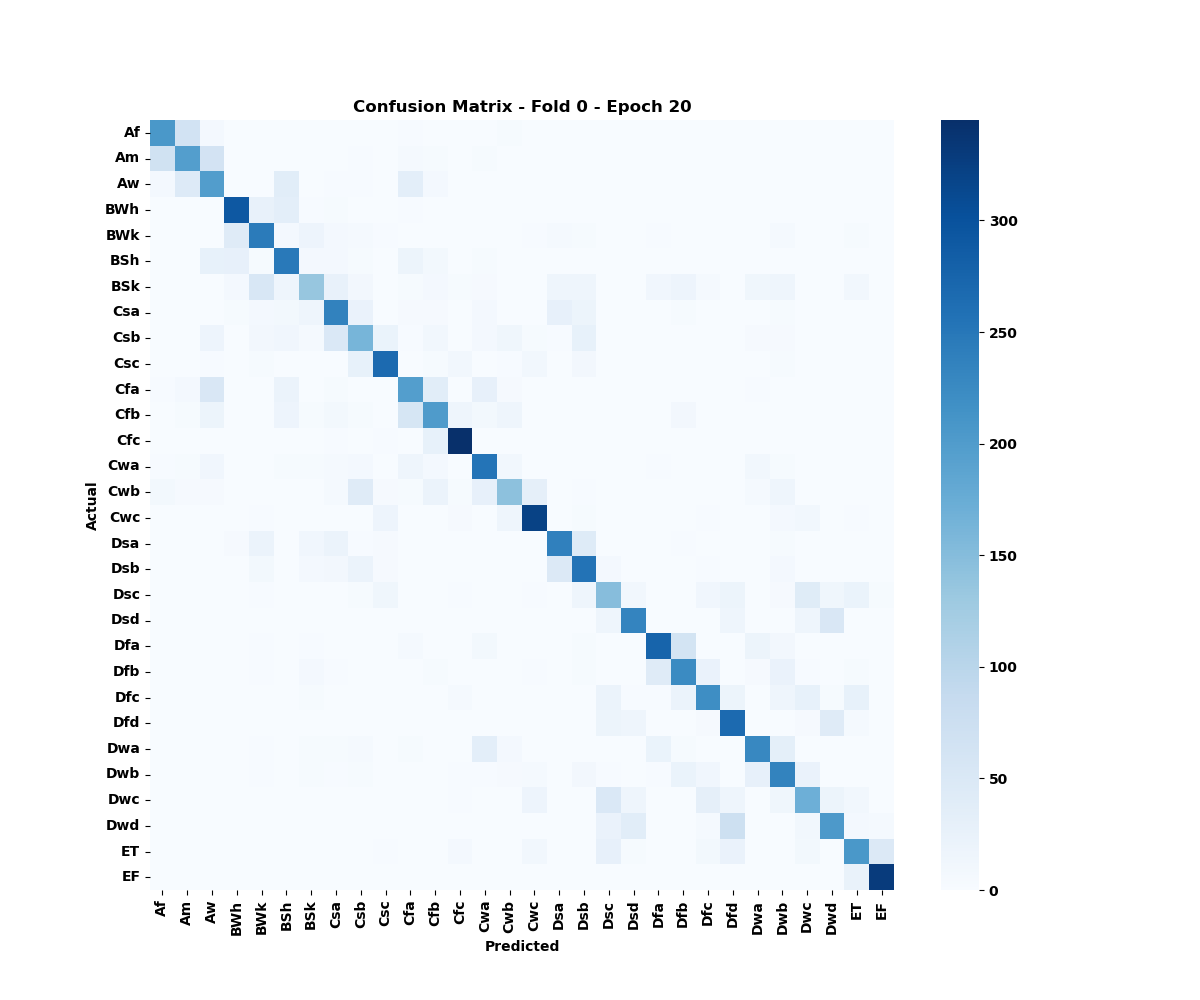
\includegraphics[width=\textwidth]{../model/final_plots/ClimateCNN_cm}
    \caption{Confusion Matrix}
  \end{subfigure}
  \hfill
  \begin{subfigure}{0.48\textwidth}
    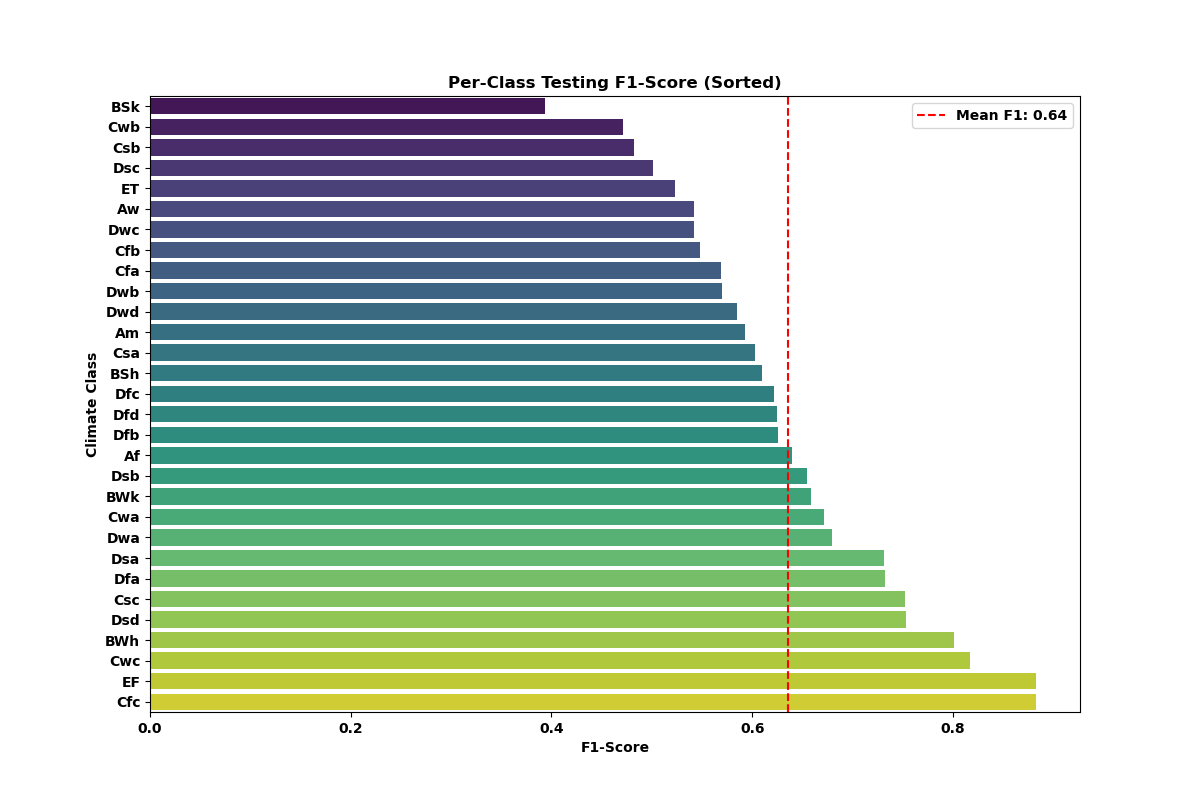
\includegraphics[width=\textwidth]{../model/final_plots/ClimateCNN_f1_score}
    \caption{F1-Scores on Testing Data}
  \end{subfigure}
  \hfill
  \begin{subfigure}{0.7\textwidth}
    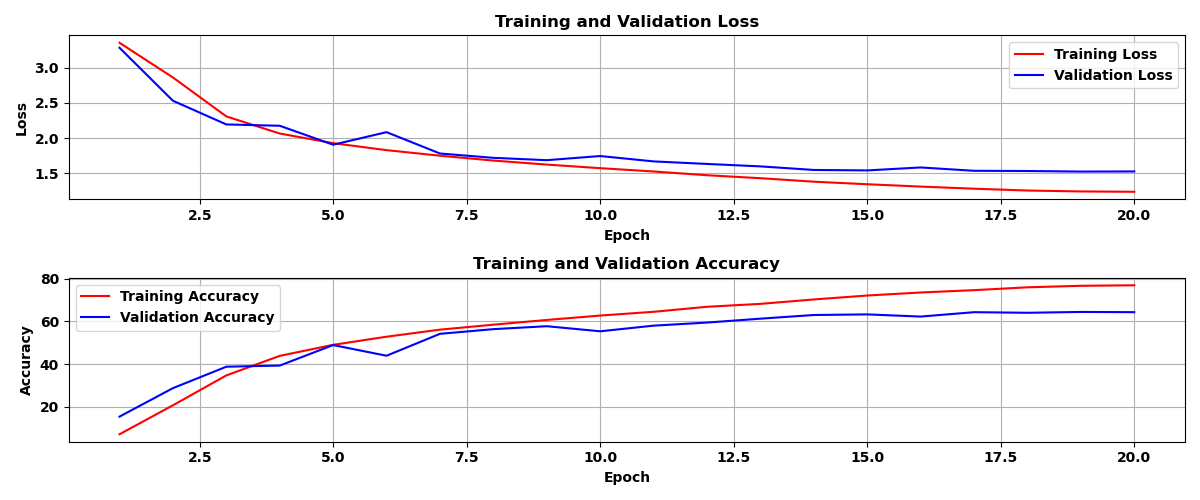
\includegraphics[width=\textwidth]{../model/final_plots/ClimateCNN_loss_accuracy}
    \caption{Loss/Accuracy}
  \end{subfigure}
  \caption{CNN Training and Evaluation Results (Epoch 20).}
  \label{fig:cnn-results}
\end{figure}

The CNN model achieved a final validation accuracy of about 64.4\%, with the mean F1-score falling at about 64\%.
With F1-score representing the harmonic mean of recall and precision, this suggests that the model is relatively good at balancing detection of class instances with minimizing false predictions, especially considering the number of classes.
The strong diagonal on the confusion matrix also shows that the model correctly classifies the majority of samples.

We additionally implemented an alternative CNN architecture that replaces the first convolutional layer of kernel size 7 with 3 layers of kernel size 3.
This keeps the same receptive field, but reduces the number of parameters and potentially allows the model to capture more non-linearity in the data.
However, the experimental results were nearly identical to the first architecture with no noticeable reduction in training time.

\subsection{Vision Transformer}
\label{subsec:vit-architecture}
In more recent years, ViT architectures have been shown to perform exceptionally well and comparably to CNN architectures for image classification tasks.
For this reason, we chose to implement a ViT model for climate classification to compare to our CNN architecture.
We built our model off of the Swin-T transformer, which is the smallest version of the Swin (Shifted Window) transformer.
This model builds hierarchical feature maps out of image patches similar to CNNs, making it a prime choice for comparison.
Transformer architectures are very data hungry, and therefore to reduce overfitting we introduce dropout (p=0.2) as well as decrease the number of decoder layers.
Similar to the CNN, we also adapt the input and output layers of the transformer for our input tensors and 30-class output.

We trained the Swin Transformer using the same K-fold cross validation and data augmentation strategies as we used for the CNN model.
The transformer architecture continued to show improvements past epoch 20, leading us to increase the total number of training epochs to 30.
This also gave us reason to keep the learning rate at 0.0001 despite the increased sensitivity of this model to higher learning rates.
Using a lower learning rate and training for a larger number of epochs would have significantly increased the training time, which would not have been feasible given our hardware restrictions.
Figure~\ref{fig:swin-results} below shows the final plots for the best fold.

\begin{figure}[H]
  \centering
  \begin{subfigure}{0.48\textwidth}
    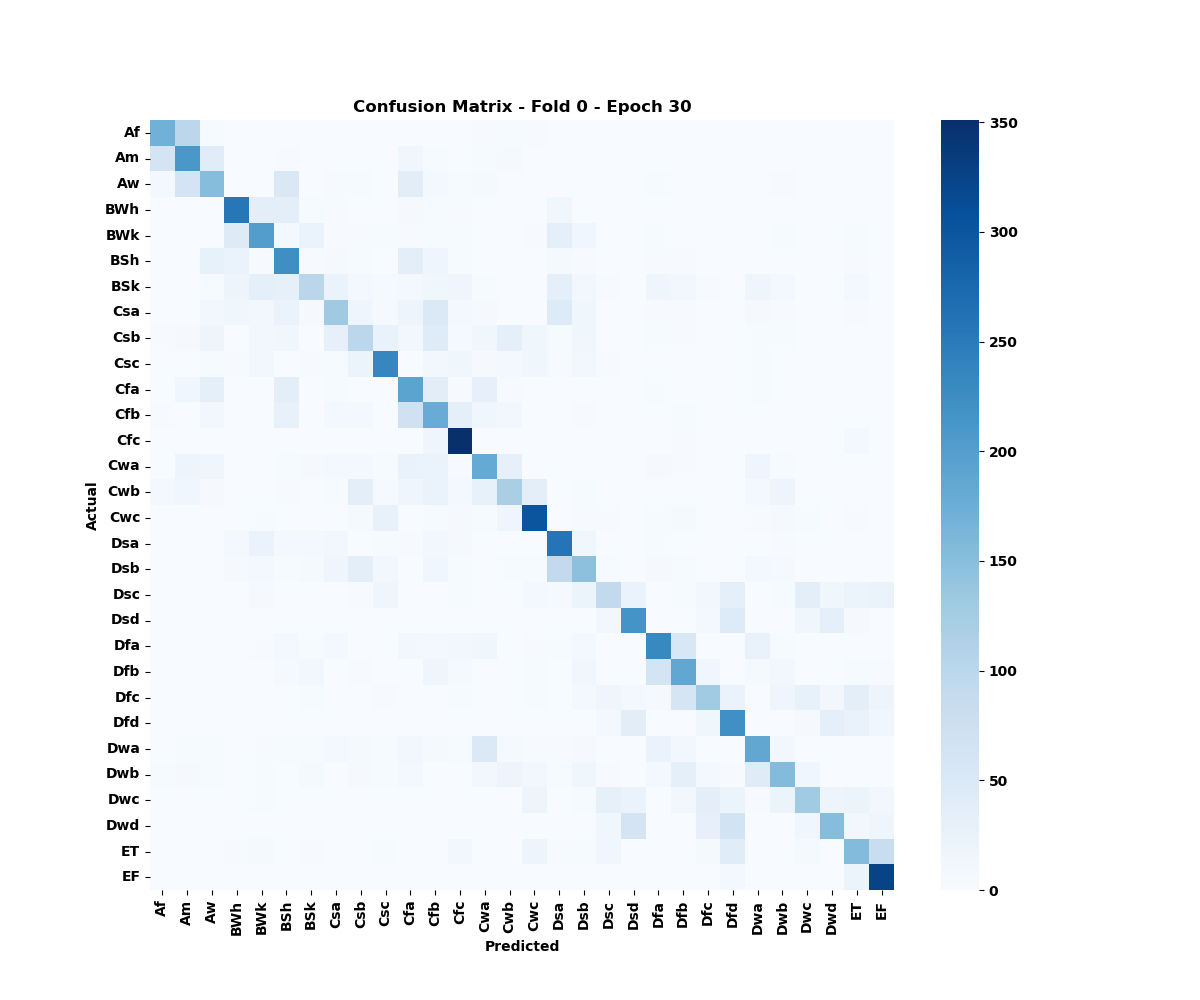
\includegraphics[width=\textwidth]{../model/final_plots/SwinTransformer_cm}
    \caption{Confusion Matrix}
  \end{subfigure}
  \hfill
  \begin{subfigure}{0.48\textwidth}
    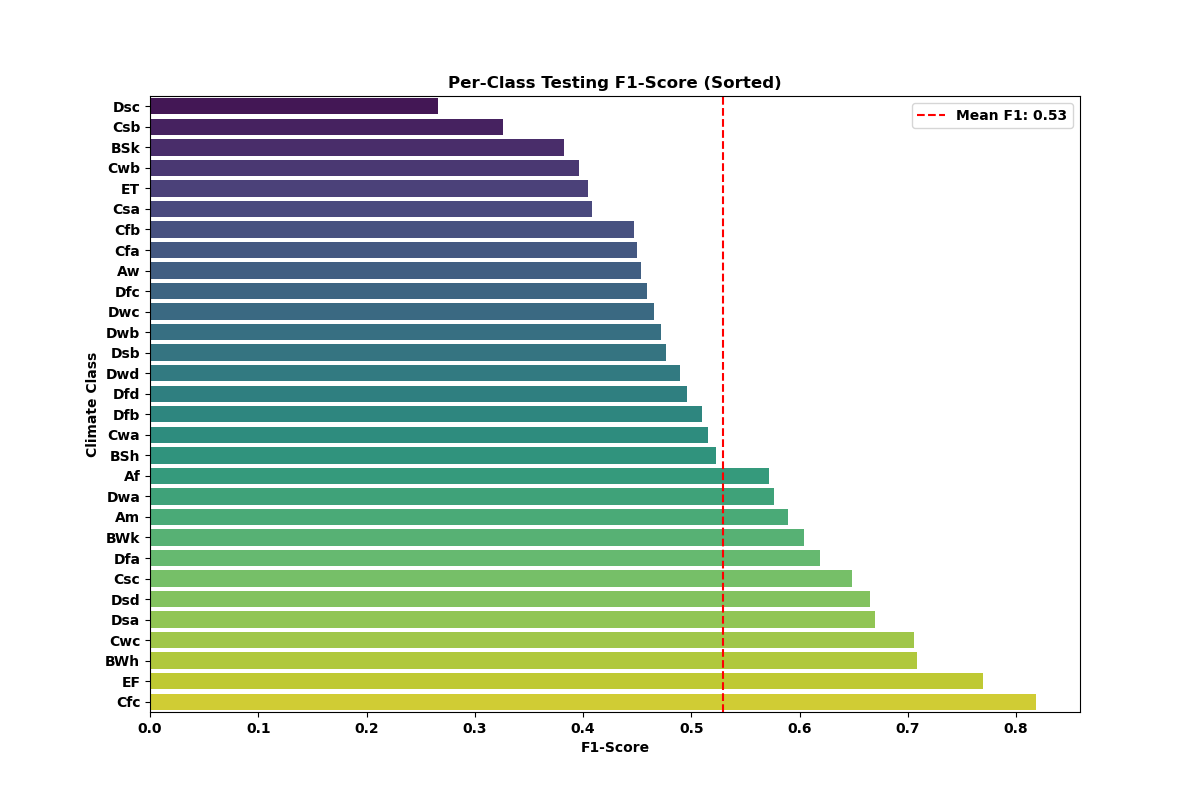
\includegraphics[width=\textwidth]{../model/final_plots/SwinTransformer_f1_score}
    \caption{F1-Scores on Testing Data}
  \end{subfigure}
  \hfill
  \begin{subfigure}{0.7\textwidth}
    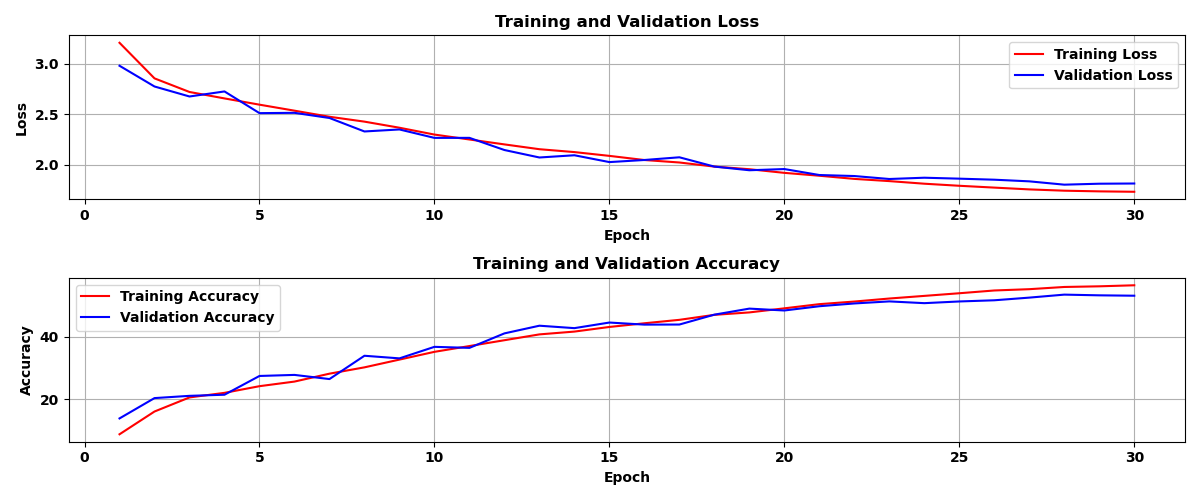
\includegraphics[width=\textwidth]{../model/final_plots/SwinTransformer_loss_accuracy}
    \caption{Loss/Accuracy}
  \end{subfigure}
  \caption{Swin Transformer Training and Evaluation Results (Epoch 30).}
  \label{fig:swin-results}
\end{figure}

The Swin Transformer achieved a final validation accuracy of about 53.4\%, with the mean F1-score falling at about 53\%.
The strong diagonal on the confusion matrix also appears comparable to that of the CNN model.

\section{Discussion (Results \& Analysis)}
\label{sec:results-analysis}
By examining the performance metrics of the different model architectures, it is clear that the deeper models (the CNN and the Swin Transformer) are the best performers.
The inclusion of models such as logistic regression, SVM, and ensemble methods serve mostly to show that the spatial features of the Sentinel-2 spectral data are indeed important for climate classification.
These simpler models do not capture these spatial features, and perform significantly worse than the CNN and  ViT architectures.
We therefore focus our analysis on the more complex architectures.

Before evaluating the performance of the CNN and Swin Transformer, it is important to establish an idea of what a ``good'' classification accuracy score looks like for this task.
The work done by \textcite{kg-climate-maps} in designing Köppen-Geiger climate classification maps using decades of climatology data serves as the gold-standard for this task.
Their research utilizes temperature and precipitation data, which are direct variables used in the Köppen formula, to generate a modern climatological map of climate classes.
When comparing their map to the ground-truth classes calculated from temperature and precipitation data sourced directly from 25,640 weather stations, they reported a classification accuracy of 80.0\% across all 30 classes.

As opposed to predicting climate classes directly from climatology data, our models are inferring climates based on Sentinel-2 spectral data that hopefully allows them to capture enough vegetation and landscape features to make accurate predictions.
Given this context, the roughly 65\% classification accuracy of our CNN model is a very good result.
Without access to the direct variables of the Köppen formula, the model was still able to learn complex climate-vegetation associations.
It is also worth noting that certain climate classes have nearly identical satellite reflectance signatures during certain times of year.
Including one example per month of the year for each sample in our dataset could help to address this issue.
However, this model still proves to be an excellent tool for addressing the issue of classifying climates in regions where temperature and precipitation data is inaccessible.
In these cases, calculating the ground-truth classes is very difficult or impossible, while our model relies only on spectral data that can be easily captured for any location on the planet.
The confusion matrix results also indicate that many of the incorrectly classified examples are predicted as classes that are close to the ground-truth class (higher density near the diagonal).
Thus, the model is still able to provide some insights about the climate class even in cases where it is not entirely correct.

In comparison to the CNN, the ViT performs similarly well for the ``easy'' classes.
The F1-score plots are very similar for the classes with the highest scores, but the Swin Transformer performs less well on the classes with the lowest scores.
Given that transformer architectures typically require millions of training examples to outperform other architectures like CNNs, this result is not surprising.
Even with the reduction in the number of decoder layers, the Swin Transformer model is still too complex for our limited dataset.
Despite this, the ViT performs considerably well, outperforming all the simpler models.
With a much larger dataset, it is likely that this model would perform equally well or better than the CNN model.

\section{Future Work}
\label{sec:future-work}
In the future, this project could benefit from various improvements.
Collecting other types of data, such as time series data, would introduce temporal features that would help our models achieve a more granular understanding of a certain area's climate behavior over different periods of time, rather than just taking a single snapshot of that area from a single season.
In addition, the ViT aspect of our project would show the most promising results, as it lacks an inductive bias like with CNNs, so synthesizing vast amounts of new data in the same manner that we did our current data would benefit its immense data needs.

\printbibliography

\end{document}
